% CU CS5525
% Fall 2012
% Python Compiler
%
% report.tex
% Semester Project Report
%
% Repository:
%    https://github.com/asayler/CU-CS5525-PythonCompiler
%
% By :
%    Anne Gatchell
%       http://annegatchell.com/
%    Andy Sayler
%       http://www.andysayler.com
%    Michael (Mike) Vitousek
%       http://csel.cs.colorado.edu/~mivi2269/

\documentclass[11pt,twocolumn]{article}

\usepackage[text={6.5in, 9in}, centering]{geometry}
\usepackage{graphicx}
\usepackage{url}
\usepackage{listings}
\usepackage{hyperref}
\usepackage{biblatex}
\usepackage{amssymb}
\bibliography{refs}

\hypersetup{
    colorlinks,
    citecolor=black,
    filecolor=black,
    linkcolor=black,
    urlcolor=black
}

\lstset{
  language={},
  basicstyle=\footnotesize,
  numbers=left,
  numberstyle=\tiny,
  stepnumber=1,
  numbersep=5pt,
  showspaces=false,
  showstringspaces=false,
  showtabs=false,
  tabsize=4,
  captionpos=b,
  breaklines=true,
  breakatwhitespace=false,
  frame=single,
  frameround=tttt
}

\lstdefinelanguage{llvm}{
  morecomment = [l]{;},
  morestring=[b]'', 
  sensitive = true,
  classoffset=0,
  morekeywords={
    define, declare, global, constant,
    internal, external, private,
    linkonce, linkonce_odr, weak, weak_odr, appending,
    common, extern_weak,
    thread_local, dllimport, dllexport,
    hidden, protected, default,
    except, deplibs,
    volatile, fastcc, coldcc, cc, ccc,
    x86_stdcallcc, x86_fastcallcc,
    ptx_kernel, ptx_device,
    signext, zeroext, inreg, sret, nounwind, noreturn,
    nocapture, byval, nest, readnone, readonly, noalias, uwtable,
    inlinehint, noinline, alwaysinline, optsize, ssp, sspreq,
    noredzone, noimplicitfloat, naked, alignstack,
    module, asm, align, tail, to,
    addrspace, section, alias, sideeffect, c, gc,
    target, datalayout, triple,
    blockaddress
  },
  classoffset=1,
  morekeywords={
    fadd, sub, fsub, mul, fmul,
    sdiv, udiv, fdiv, srem, urem, frem,
    and, or, xor,
    icmp, fcmp,
    eq, ne, ugt, uge, ult, ule, sgt, sge, slt, sle,
    oeq, ogt, oge, olt, ole, one, ord, ueq, ugt, uge,
    ult, ule, une, uno,
    nuw, nsw, exact, inbounds,
    phi, call, select, shl, lshr, ashr, va_arg,
    trunc, zext, sext,
    fptrunc, fpext, fptoui, fptosi, uitofp, sitofp,
    ptrtoint, inttoptr, bitcast,
    ret, br, indirectbr, switch, invoke, unwind, unreachable,
    malloc, alloca, free, load, store, getelementptr,
    extractelement, insertelement, shufflevector,
    extractvalue, insertvalue,
  },
  alsoletter={\%},
  keywordsprefix={\%},
}

\newenvironment{packed_enum}{
\begin{enumerate}
  \setlength{\itemsep}{1pt}
  \setlength{\parskip}{0pt}
  \setlength{\parsep}{0pt}
}{\end{enumerate}}

\newenvironment{packed_item}{
\begin{itemize}
  \setlength{\itemsep}{1pt}
  \setlength{\parskip}{0pt}
  \setlength{\parsep}{0pt}
}{\end{itemize}}

\newenvironment{packed_desc}{
\begin{description}
  \setlength{\itemsep}{1pt}
  \setlength{\parskip}{0pt}
  \setlength{\parsep}{0pt}
}{\end{description}}

\begin{document}

\title{
  Building a LLVM Python Compiler
}

\author{
  Anne Gatchell    \\ \texttt{anne.gatchell@colorado.edu} \and
  Andy Sayler      \\ \texttt{andrew.sayler@colorado.edu} \and
  Michael Vitousek \\ \texttt{michael.vitousek@colorado.edu}
}

\date{\today}

\maketitle

\begin{abstract}

We discuss the expansion of our P3 compiler to target LLVM intermediate
language assembly code. This involves converting our intermediate
AST to SSA form as well as replacing the instruction selection
components of the existing compiler. We compare the performance and
flexibility of directly targeted x86 code vs targeting LLVM IR code.

\end{abstract}

\section{Problem Statement}

While the existing HW6, p3-compliant compiler supports 32-bit, x86
code generation, it does not support generating code for the variety
of non-x86 architectures and assembly languages common today (x64,
ARM, etc). While we could remedy this deficiency by adding additional
native code generation for non-x86 architectures directly to our
compiler, this approach would duplicate a wide range of existing
effort and would require continued maintenance to support new
architectures and assembly languages as they arise. From a software
engineering perspective, such an attempt would also increase the
likelihood of bugs and errors due to the expanded code base and much
larger required breadth of expertise in a variety of assembly
languages.

Instead, we aim to leverage the existing work done by the LLVM project
\cite{llvm.org} to convert our HW6 compiler from an x86-targeted
compiler to an LLVM-targeted compiler. This will not only be efficient
from a maintenance standpoint, but it will also be a useful
introduction to a modern, commonly used compiler intermediate
language. We will maintain the current x86 targeting and add LLVM IR
Assembly \cite{lattner-llvmlangref} as an additional targeting
option. In this way, we will be able to compare our natively generated
x86 code with the LLVM-assembler generated x86 code. We will also be
able to experiment with compiling our LLVM byte-code files to assembly
languages other than x86 such as x64 and ARM.

LLVM is quickly becoming the de facto standard target for most modern
compilers for high level languages.  It provides multi-platform
support, multi-runtype support (compiled, interpreted, JIT compiled,
etc), and access to a range of existing optimization tools and
techniques. Through this project, we hope to become familiar with the
LLVM Assembly Language and LLVM system architecture while gaining
insight into the benefits of building an LLVM-targeted compiler.

\section{Background}

The primary change to our existing compiler code base is the addition
of an LLVM output target option. We discuss LLVM and its prerequisites
in this section.

\subsection{LLVM}

The Low Level Virtual Machine (LLVM) is an open source project that
was initially intended to provide support for a Static Single
Assignment (SSA) compiler that is capable of statically or dynamically
compiling any programming language \cite{llvm.org}.

The LLVM project specifies a standardized Intermediate Representation,
essentially a platform-agnostic assembly language, in which programs
can be written. Listing \ref{lst:llvm-example_hello0.ll} shows
a simple LLVM hello world program as an example of
what LLVM IR Assembly language looks like.

\lstinputlisting[
  float=*htb,
  language=llvm,
  label=lst:llvm-example_hello0.ll,
  caption={LLVM Assembly - Hello World Example \cite{lattner-llvmlangref}}
]{../code/llvm-examples/hello0.ll}

The LLVM IR language exists in three grammatically equivalent forms:
as an in-memory data structure, as a human readable ``assembly''
language, and as an file-oriented bitcode (.bc) \cite{lattner-llvmlangref}.
Converting between these three forms is handled via the various tools
in the LLVM tool chain. Listing \ref{lst:llvm-example_hello0.ll} is an
example of the human-readable form presented in the examples in this paper.

While LLVM IR is more
flexible in terms of multi-platform support, its
general syntax is more stringent than lower level assembly languages
like Intel x86. For example, unlike x86, LLVM IR is a typed language.
Each instruction must list the types of all arguments involved. When
data must be converted from one type to another, explicit casting
operations must be used. No loose or implicit casting is allowed.

Another requirement of LLVM IR, and a corollary of the typed nature of
LLVM IR, is that all functions used in a LLVM IR file must provide
explicit prototype definitions in the file. This included calls to
external functions that will be linked into the program during
compilation. This requires that every LLVM IR file have access to a
complete list of function prototypes for any library or other external
functions it wishes to use. This list is necessary so that the LLVM
build-chain can enforce the LLVM types at every stage in the build
process.

LLVM requires Static Single Assignment (SSA) form. This means that
each variable/register in an LLVM IR program can only be
written/assigned to once. SSA form is discussed detail in the Section
\ref{sec:SSAForm}.

Related to the SSA requirement, LLVM IR does not allow direct
assignments. Registers may only be used on the RHS of a statement if
they are arguments to a specific operation. For example, the statement:
\begin{verbatim}
x = input()
y = x
print(y)
\end{verbatim} 
is not allowed. Instead, the \texttt{y = x} assignment must be
eliminated and the \texttt{x} register propagated forward to a point
where it is read as an argument to an operation. Since LLVM IR must be
in SSA form, eliminated direct assignments becomes a simple
``find+replace'' issue. Thus, the previous example needs to be
converted to:
\begin{verbatim}
x = input()
print(x)
\end{verbatim}
before it can be compiled to valid LLVM IR.

Finally, all LLVM IR statements must be organized into strictly
defined control ``blocks''. Each block starts with a label (although
this label can be emitted from the first block in a function) and end
with one of a small set of ``terminator'' instructions such as
\texttt{ret}, \texttt{br}, or \texttt{switch}. In LLVM IR, unlike in
x86, you can not ``fall through'' one block to the next without using
an explicit terminator instruction specifying a jump to the next
blocks label. This strictly-defined block-based organization
requirement allows the LLVM tool chain to construct a well defined
flow graph through the LLVM code. Listing \ref{lst:blocks.ll} shows an
example of a short LLVM IR program containing a series of blocks with
labels at the start of each block and explicit branching at the end of
each block.

\lstinputlisting[
  float=*htb,
  language=llvm,
  label=lst:blocks.ll,
  caption={LLVM Assembly - ``Block'' Example}
]{./include/ll/blocks.ll}

\subsection{Static Single Assignment Form}
\label{sec:SSAForm}

A program is in SSA form when its variables are assigned exactly once
in the program \cite{gcc-gnu.org}. Most programs are not written in an
SSA form, but can be converted to SSA form by giving a variable a new
name every time it is assigned to, and replacing all uses of the
variable in right-hand side expressions with the most recent version
of the variable \cite{brandis-mossenbock}. In a linear code segment,
this is a fairly straightforward transformation. When branching and
polymorphism are added, however, it becomes a more complex issue, as
seen below:

\begin{verbatim}
if input():
  x = 3
else:
  x = 3.145
print x
\end{verbatim}

This piece of code contains branching, so x is being assigned to
multiple times. In addition, x could be an integer or a floating point
number. To convert to SSA in this situation, compilers can add a
\emph{phi} ($\phi$) node to select the proper version of x to use as
the current version. See below:

\begin{verbatim}
if input():
  x_0 = 3
else:
  x_1 = 3.145
x_2 = PHI<x_1, x_2>
print x_2
\end{verbatim}

The $\phi$ function (node) serves to pick the branch that was used at
runtime, and return that version of x.

Fortunately, LLVM provides a \emph{phi} node in its assembly language
specification \cite{lattner-llvmlangref}. It addresses the multiple
assignment problems that result from control flow. The syntax is

\begin{verbatim}
<result> = phi <ty> [<val0>, <label0>]...
\end{verbatim} 

where the ``ty'' field is the incoming type of the data to be chosen
from. However, this indicates that the $\phi$ node can not handle
explicit polymorphism. Fortunately, we have already packaged all of
our data types into one unique type: a pyobj. All values passed to the
block must be first class values, so a pointer to a pyobj will be the
only option available to handle polymorphism. The type field is
followed by a list of pairs, one for each predecessor block of code in
the current block, and the $\phi$ function will use the value
corresponding to the block actually executed.

\section{Approach}

Prior to actually modifying our compiler, we spent extensive time
manually experimenting with LLVM Assembly. This included manually
``compiling'' several of our test programs to LLVM assembly, and then
compiling and running the LLVM Assembly we produced, in order to
verify our understanding of the language. This process both increased
our understanding of the LLVM language, and allowed us to create the
updated build and test infrastructure for LLVM files.

After familiarizing ourselves with LLVM, we proceeded to modify our
compiler via the following development steps:

\begin{packed_enum}
\item Fixed bugs in existing compiler until we passed all valid student
  and instructor provided p3 test cases.
\item Re-factored existing compiler to better handle common visitor
  functions, support a modular parser-interface, and reduce code
  complexity.
\item Added an additional compilation pass that translates the flattened
  AST into SSA form.
\item Added an alternate instruction selection pass that generates LLVM
  assembly instead of x86 assembly.
\item Added the necessary top-level compiler control handling to switch
  between LLVM and x86 generation based on an input parameter.
\item Modified the existing Makefile, build, and test systems to handle
  both x86 and LLVM code generation. Converted test infrastructure to
  performing 3-way compares between native Python execution, x86
  execution, and LLVM execution.
\item Confirmed behavior of LLVM generated code matches that of the
  native Python interpreter, as well as that of the x86 generated
  code.
\item Identified and fixed bugs as necessary.
\end{packed_enum}

\section{Design}
\label{sec:design}

Our compiler design begins with the basic compiler design presented in
\cite{siek-chang} for the Python ``P3'' language subset.  We then
proceeded to re-factor this design to better exploit code reuse,
remove deprecated interfaces, support multiple target types, and
automatically catch a range of implementation errors. We kept the re-factored design common for all compilation targets
through the end of the flatten pass.

The major changes happen after flatten in the instruction selection
and related passes. A significant difference between our current x86
compiler and our LLVM compiler is that the LLVM compiler requires the
AST to be in SSA form. In addition, LLVM uses variable names, not
pre-defined registers, in its instructions. As such, the LLVM
compilation requires an additional pass to convert to SSA form, but
can forgo the pass that performs register allocation, since the LLVM compiler performs register allocation during its compilation of the bitcode. An alternate version of the instruction selection pass has also been added in support of to the LLVM Assembly format.

\subsection{Module Flow}
\label{sec:ModuleFlow}

\begin{figure*}[htb]
   \centering
   \includegraphics[width=.90\textwidth]{./include/CompilerFlow.pdf}
   \caption{Compiler Data Flow}
   \label{fig:CompilerFlow}
\end{figure*}

Our compiler employs a modular design to maximize code reuse between
various target languages.  Our compiler stages up through flatten are
designed to be target-agnostic. It is only the post-flatten stages
that differ based on the compilation target (x86 or LLVM). Figure
\ref{fig:CompilerFlow} shows our modular flow through our compiler and
the various data structures present between each stage.

The new compiler stages necessary for LLVM targeted compilations are
the ``SSA'' stage, the ``Propagate'' stage, and the ``LLVM Instruction
Selection'' stage. The purpose of each stage is briefly discussed
below.

\begin{packed_desc}
\item[SSA Stage] \hfill \\
  The Static Single Assignment (SSA) stage converts
  the multi-assignment Python AST into a Static Single Assignment
  Python AST. It replaces variable assignments to ensure each variable
  is only ever written once, and also sets up the necessary Phi operations
  associated with branching nodes (if, while, etc).
  This process is discussed further in Section \ref{sec:stage-SSA}.
\item[Propagate Stage] \hfill \\
  The propagate stage is essentially a
  lightweight constant propagation stage. Its goal is to eliminate
  all direct assignments (i.e. \texttt{|x = y|}) in favor of propagating
  the right hand side of such assignments into the actual operation in
  which they are used (i.e. \texttt{|x = y; print(x)|} $\rightarrow$
  \texttt{|print(y)|}). Since the code is already in SSA form, this
  process involves a rather simple search and substitution algorithm
  This process is discussed further in Section \ref{sec:stage-Propagate}.
\item[LLVM Instruction Selection] \hfill \\
  The LLVM Instruction Selection stage
  converts the Python AST into an LLVM IR (assembly) AST. The biggest
  challenge in this stage is converting the multi-branches Python AST
  into the linear list of code ``blocks'' that LLVM IR requires. This
  process is discussed further in Section
  \ref{sec:stage-LLVMInstructionSelection}.
\end{packed_desc}

We have also created a new initial compiler pass that converts the AST
nodes from whatever format a given parser outputs to a uniform set of
internal AST nodes used throughout the rest of the compiler. This
allows us to switch parsing infrastructures without needing to change
the core compiler code. We have leveraged this capability to move away
from the deprecated Python ``compiler'' package used for the course
assignments thus far in favor of the built-in AST and parsing
infrastructure inherent in Python 2.7+.

\subsubsection{SSA}
\label{sec:stage-SSA}

LLVM requires Static Single Assignment form, meaning that each
variable is assigned to exactly once.  We convert programs into SSA
form during compilation (only when compiled to SSA --- our x86
compiler does not utilize the SSA conversion module), a process which
occurs after flattening and before LLVM instruction
selection (as shown in Figure \ref{fig:CompilerFlow}).  This
conversion process takes a single pass over the program, and converts
it as follows:

\begin{itemize}
\item When an assignment statement (to a variable) is encountered, the
  converter increments the ``version number'' of the variable (or
  initializes it to $0$ if the variable has not been previously
  assigned to). The variable is then renamed to record this version
  number, and the current version number of the variable is recorded
  in a dictionary.
\item When a variable name is encountered, it is replaced by the most
  recent version of the variable.
\item When an If statement is encountered, the true and false branches
  are scanned for their assigned variables, and a new attribute is
  added to the end of the statement, containing Phi nodes for the
  variables assigned within the If as follows:
  \begin{itemize}
  \item If a variable is assigned to in both branches, the Phi node
    contains the version from each branch.
  \item If a variable is assigned to in one branch but not the other,
    \textit{and} the variable was also assigned to before the If
    statement was entered, then the Phi node contains the new version
    in the branch it appeared in, and the old version in the other
    branch.
  \item If a variable is assigned to in one branch but not the other,
    \textit{and} the variable did not exist before the If
    statement was entered, no Phi node is created for it.
  \end{itemize}
\item When a While loop is encountered, its body is scanned for
  assigned variables. A new attribute is then added to the beginning
  of the statement, containing Phi nodes for each variable that is
  assigned to in the body and that also existed before the loop was
  entered.
\end{itemize}

This process ensures that each variable is assigned to only once while
maintaining the semantics of the program. At the moment, we do not use
any of the optimizations, such as those based on computing the
dominator tree of the program as described by Brandis and
M\"{o}ssenb\"{ock} \cite{brandis-mossenbock}, though we may implement such
optimizations in the future, especially if the conversion pass is
moved to an earlier point in the compilation.

\subsubsection{Propagate}
\label{sec:stage-Propagate}

The propagate stage eliminates direct assignments from the code (which
are not legal in LLVM) in favor of propagating the right-hand-side of
such assignments all the way to the point at which they are used in an
operation. 

For example, the code shown in Listing \ref{lst:direct_assignment.ll}
is not legal LLVM IR code. The correct, ``propagated'' version is
shown in Listing \ref{lst:direct_assignment_fixed.ll}.

\lstinputlisting[
  float=*htb,
  language=sh,
  label=lst:direct_assignment.ll,
  caption={A Direct Assignment Operation (Not Legal LLVM IR)}
]{./include/ll/direct_assignment.ll}

\lstinputlisting[
  float=*htb,
  language=sh,
  label=lst:direct_assignment_fixed.ll,
  caption={The ``propagated'' version of Listing
    \ref{lst:direct_assignment.ll} (Legal LLVM IR)}
]{./include/ll/direct_assignment_fixed.ll}

The propagate pass is designed to operate on a Python AST in SSA
form. Thus, it immediately succeeds the SSA stage. Since the code is
already in SSA form, the propagate stage can perform a simple
``find-and-replace'' algorithm on all variable names in the AST. The
algorithm is implemented as a set of visitors corresponding to Python
AST nodes. The basic logic is:

\begin{packed_enum}
\item Create an empty global dictionary for mapping LHS variable names
  to RHS variable names
\item Traverse the AST
\item When a variable assignment node is found, check to see if the
  RHS is a pure variable (i.e. not larger expression node)
  \begin{packed_enum}
  \item If it is:
    \begin{packed_enum}
    \item Check to see if the LHS variable is a key in the
      global dictionary. If it is, replace the LHS variable with the
      value associated with the key in the global dictionary
    \item Add the RHS:LHS variable mapping to the global dictionary
    \item Remove the node from the tree
    \end{packed_enum}
  \item If it is not:
    \begin{packed_enum}
      \item Do nothing
    \end{packed_enum}
  \end{packed_enum}
\item When a variable name is encountered, check to see if the name is
  a key in the global dictionary. If so, replace the name with the
  value associated with this key.
\item When a branching statement node (If, While, etc) is encountered,
  search the associated Phi list for any variables that are keys in
  the global dictionary, and replace them with the corresponding
  values as necessary.
\end{packed_enum}

\subsubsection{LLVM Instruction Selection}
\label{sec:stage-LLVMInstructionSelection}

The LLVM Instruction Selection stage converts the Python AST to an LLVM
AST. The primary challenge in this stage is messaging our Python AST
into a format that meets the rather strict LLVM requirements. We must
also substitute one or more LLVM AST nodes for each Python AST node
while maintaining the semantics of the program.

% Discuss Typing Approach

The first challenge that must be dealt with in instruction selection
is dealing with the LLVM IR's strict typing requirements. Fortunately,
our use of pyobj pointers will make this process fairly simple. In
effect, the only variables used in our program are pyobj pointers,
ints, bools, and bigpyobjs. Do to the design of the helper functions,
all of these types can be treated as either 32-bit ints (on a 32-bit
system) or 64-bit ints (on a 64-bit system). This allows us to
effectively deal with a single type throughout our entire LLVM IR
program. Thus we can assume that all of are function arguments,
variables, etc are of this single type and avoid needing to track
variable and function types explicitly.

There are a few points where this single type assumption breaks down,
namely when using the LLVM compare operator (which only returns
bool-like 1-bit integers) and when making indirect function calls
(where explicit function pointer types are required). Fortunately, the
situations where these alternate types arise are well isolated in the
LLVM IR code, and always result from the mapping of a single Python
AST node to sever LLVM IR nodes. These alternate types are also able
to be cast back and forth to 64 or 32 bit integers, matching the
single type used throughout the rest of the code. Thus, we can simply
insert the necessary casting operations to convert these types to or
from the default type when we generate the code that requires these
special types. 

% Discuss Function Prototype Declaration Approach

We must also deal with the fact that all LLVM IR files must include a
list of prototype definitions for any external library functions we wish
to call. In the case of our compiler, these external function or
limited to the list of runtime helper functions specified in
\texttt{runtime.h}. To deal with this requirement, we created an LLVM
IR file that contains the necessary LLVM declarations for each
\texttt{runtime.h} function
\footnote{Technically, we have two version
  of this file: one which contains the \texttt{runtime.h} LLVM
  function declarations using 64-bit integers as the single generic
  type (for use on 64-bit systems), and one which contains the
  \texttt{runtime.h} LLVM function declarations using 32-bit integers
  (for use on 32-bit systems). Our compiler detects the bit-width of
  the system on which it is running and dynamically selects the correct
  file at compile time}.
The contents of this file is then
pre-pended to the LLVM IR output our program generates as part of
the process involved in writing the compiled LLVM AST to a file. A
small snippet of this file is shown in Listing
\ref{lst:runtime-declares-x64.ll}.

\lstinputlisting[
  float=*htb,
  language=sh,
  firstline=1,
  lastline=11,
  label=lst:runtime-declares-x64.ll,
  caption={The opening snippet of the LLVM \texttt{runtime.h} function
  declaration file}
]{../code/helper/runtime-declares-x64.ll}

% Discuss ``Blocking'' Approach

To Do...

% Discuss LLVM AST Operation Mapping Approach

To Do...

\subsection{LLVM Build Process}

We have also implemented a method for compiling the C run-time helper
functions to LLVM bitcode using the LLVM front end C compiler, clang
\cite{clang.llvm.org}. We then link the helper function generated
bitcode to the bitcode generated from the .ll output from our
compiler. This gives us a bitcode file that we are capable of running
in the LLVM interpreter or fully compiling to an executable.  The
process for compiling is shown in Listing \ref{lst:compiling.sh}.

\lstinputlisting[
  float=*htb,
  language=sh,
  label=lst:compiling.sh,
  caption={Pseudo-script describing the LLVM build process}
]{./include/txt/compiling.sh}

\section{Results}

The full source code for our compiler is available at \cite{github-repo}.

Our implementation met the full standards for P3-Python, and we also
added support for the greater-than and less-than operators, in order
to expand the space of test cases and benchmarks that we could
create. In addition to compiling to the x86 architecture (in both 32
and 64 bit forms), we were able to compile to the ARM architecture and
run our compiler on an ARM-based computer (the Raspberry Pi). This was
possible due to the cross-platform nature of LLVM, and necessitated
only minor changes to our tool-chain, and none at all to our compiler
itself.

In order to compare the behavior of our compiler to that of our x86
implementation, we developed a benchmarking suite and recorded both
compilation times and runtimes. Graphs for both of these metrics are
shown in Figures \ref{fig:ct} and \ref{fig:rt}. Both graphs display a
speedup factor, with the runtime/compile time of the x86
implementation normalized to $1$. We also display the running and
compile time of an interpreted version of the test cases --- in
addition to compiling to a binary, LLVM is also capable of
interpreting bitcode files using a JIT. Finally, we also compare our
results to a native Python implementation's runtime.

\begin{figure*}[htb]
  \centering
  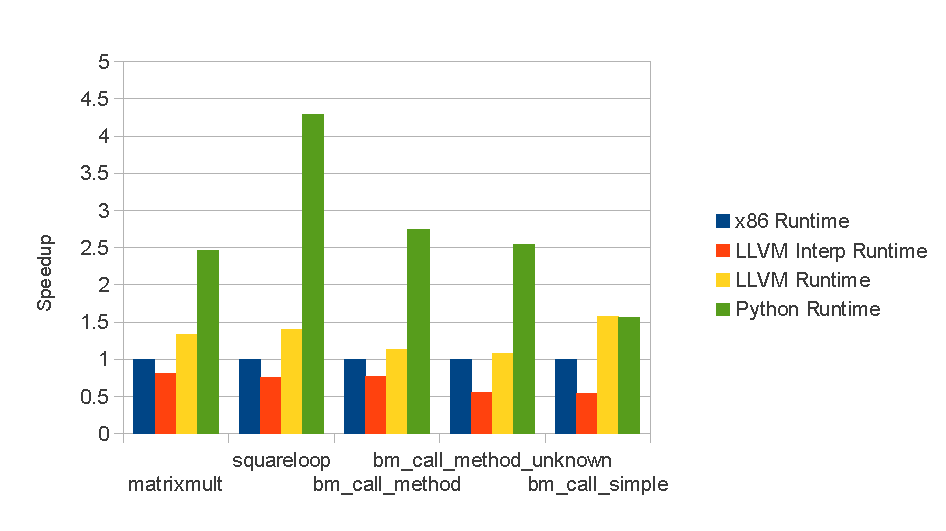
\includegraphics[scale=.9]{include/pdf/runtime.pdf}
  \caption{Runtime benchmarks.}
  \label{fig:rt}
\end{figure*}

We find that when using LLVM to fully compile our benchmarks we are
consistently faster than our previous x86 implementation at runtime,
although the degree of speedup varies, as shown in Figure
\ref{fig:rt}. The LLVM implementation is significantly faster on
benchmarks that primarily use simple function calls, loops, and math,
approaching a $1.6\times$ speedup. On the other hand, the degree of
improvement is much reduced when performing method calls and attribute
lookups. The native Python interpreter still outperforms our LLVM
interpreter on most test cases, except that it is approximately equal
to our compiler on a benchmark involving many simple function calls;
possibly this is a domain highly suited to the structure of LLVM's IR
and bitcode. Meanwhile, interpreted LLVM bitcode is consistently much
slower than either the x86 implementation or the compiled LLVM.

\begin{figure*}[htb]
  \centering
  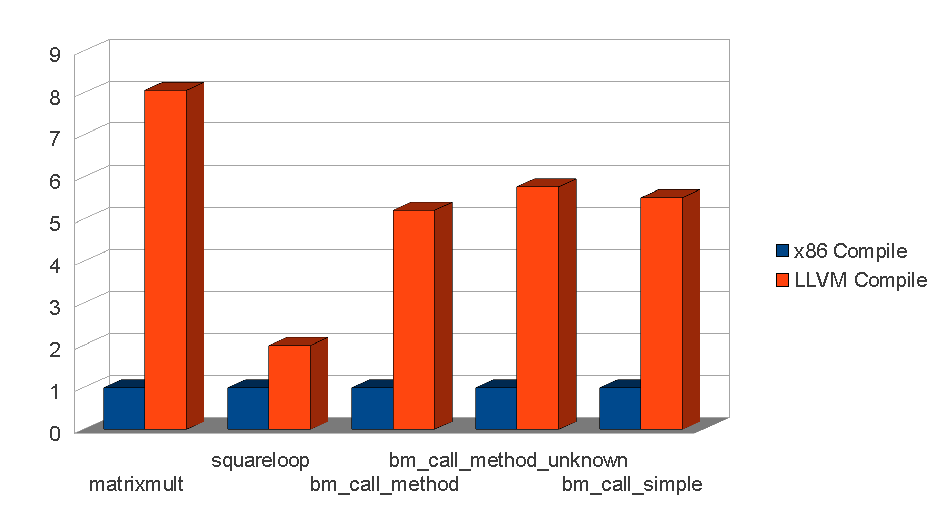
\includegraphics[scale=.9]{include/pdf/compiletime.pdf}
  \caption{Runtime benchmarks.}
  \label{fig:ct}
\end{figure*}

In terms of compile times, we see that the LLVM compiler is far faster
than the x86 compiler on all benchmarks, as shown in Figure
\ref{fig:ct}. Our benchmarking setup includes the time taken by
elements of the tool-chain besides just our own compiler, so the
timings seen here are able to be compared. We suspect that the primary
reason for the out-performance of the x86 compiler by the LLVM compiler
is that LLVM performs register allocation internally, and presumably
it is much more efficient at this process than our un-optimized
register allocator. Note also that it takes approximately half as long
to compile to LLVM bitcode as it does to compile to binaries using
LLVM; however, both the interpreter compilation and the binary
compilation process use the exact same code paths through our
compiler. This indicates that, at least in compilation to binaries
using LLVM, our compiler does not dominate the rest of the LLVM
tool-chain in terms of compilation time.

\section{Discussion}

...To be added when complete...

\section{Conclusion}

...To be added when complete...

\nocite{*}
\printbibliography

\end{document}
